\documentclass[12pt]{amsart}
\usepackage{amsmath, amsthm, amssymb}
\usepackage[margin=1.2in]{geometry}
\usepackage{hyperref}
\setlength{\textheight}{8.5in}
\setlength{\evensidemargin}{0.0in}
\setlength{\oddsidemargin}{0.0in}
\setlength{\topmargin}{-0.5in}
\setlength{\textwidth}{6.5in}

\newtheorem{theorem}{Theorem}
\newtheorem*{theorem*}{Theorem}
\newtheorem{lemma}{Lemma}
\newtheorem*{lemma*}{Lemma}

\theoremstyle{definition}
\newtheorem{definition}{Definition}

\newtheorem{corollary}[theorem]{Corollary}
\newtheorem{proposition}[theorem]{Proposition}
\newtheorem{conjecture}[theorem]{Conjecture}
\theoremstyle{remark}
\newtheorem{remark}[theorem]{Remark}

\newcommand{\Z}{\mathbb{Z}}
\newcommand{\Q}{\mathbb{Q}}

\usepackage{graphicx} % Required for inserting images

\title{Understanding the Properties of Taxicab Numbers}
\author{Samir Kadariya, Jovani Pitterson, Skyler Pulling}
\date{March 2026}

\begin{document}

\maketitle

\begin{abstract}
    Taxicab numbers are a unique category of integers that can be represented as the sum of two cubes in multiple distinct ways. By analyzing taxicab numbers, we can illuminate many properties of cubic sums and the structure of modular cubes. Within this paper, we will analyze some of the properties of taxicab numbers, including determining the second taxicab number, proving that infinitely many taxicab numbers exist, creating a generating formula for taxicab numbers, and putting bounds on the growth rate and density of the set of taxicab numbers. In doing so we form a clearer understanding of the structure of the set of taxicab numbers.
\end{abstract}

\section{Introduction}
A taxicab number is a positive integer expressible as the sum of two positive cubes in at least two distinct ways. More specifically, for this paper, we define a taxicab number as follows
\begin{definition} 
    A \textit{Taxicab Number} is any positive integer $N \in \mathbb{Z^+} $ such that there exists some $a,b,c,d \in \mathbb{Z^+}$ that satisfy the condition $a^3+b^3=N=c^3+d^3$ and that $\{a,b\} \neq \{c,d\}$. That is, $N$, can be written as the sum of $2$ algebraic cubes in at least $2$ distinct ways.
\end{definition} 
Coined by Srinivasa Ramanujan, Taxicab numbers are a topic of significant interest to number theorists for their unique structure and the insight they grant on the properties of integers cubed. Famously, Ramanujan declared $1729$ to be the first taxicab number, as it can be represented as both 
\[ 1729 = 12^3 +1^3 \text{  and   } 1729=10^3+9^3.\]

In this paper, we will discuss some of the properties of taxicab numbers that can be derived from Ramanujan's definition. First, we wish to understand how many taxicab numbers there are. By understanding the size of the set of taxicab numbers and the identity of its elements, we can make conclusions about the patterns and trends that the set follows. To determine the amount of taxicab numbers, we will start by showing that a second taxicab number exists, and verifying that there is no number between $1729$ and the found 2nd taxicab number that could satisfy the conditions to be a taxicab number. In Section $2$, we begin by proving that $4104$ is the second taxicab number. With knowledge that $4104$ is the second taxicab number, we eliminate the possibility that $1729$ is the only number that meets the conditions of a taxicab number. Now, reaching the conclusion there are multiple taxicab numbers, we shift to discussing if there are infinitely many taxicab numbers in Section $3$. \\


Having established that Taxicab numbers exist beyond $1729$, in
Section~$3$ we ask how many there are. A first observation is 
that any Taxicab number $N = a^3 + b^3 = c^3 + d^3$ generates infinitely 
many others by scaling: $t^3 N = (ta)^3 + (tb)^3 = (tc)^3 + (td)^3$ for 
any positive integer $t$. These scaled copies share the same underlying 
identity and so are considered trivially related. The more substantive 
question is whether there exist infinitely many Taxicab numbers that are 
pairwise non-trivially related and therefore not obtainable from one another 
by such scaling. We answer this by constructing a 
one-parameter family of Taxicab identities, parametrized by positive 
integers $n$, and proving that no two members of the family are rescalings 
of one another. After concluding that infinitely many classes of taxicab numbers exist, we then consider how rare taxicab numbers become at higher integer values, which we discuss in Section $4$. \\

As a result of the conclusion that there are infinitely many taxicab numbers, we now shift our consideration to establishing general growth rates and density bounds for taxicab numbers in Section $4$. In doing so, we establish how common taxicab numbers are amongst the integers and how that rarity scales as we approach larger integers. Specifically, we will use bounding arguments on the size of the set of taxicab numbers, up to some integer, to prove that the number of taxicab numbers up to any positive integer $X$ is $O(X^{2/3})$ and $\Omega(X^{1/3})$. Using additional empirical evidence, we will also conjecture a tighter lower bound that could be set on the density of the taxicab numbers. By isolating the taxi cab numbers that are not within the same taxicab number class of each other, we find a separate bound that the number of non-trivially related taxicab numbers up to any positive integer $X$ is $O(X^{2/3})$ and $\Omega(X^{1/9})$.\\

Finally, in Section 5, we analyze the modular structure of sums of two cubes to determine which residue classes can contain Taxicab numbers. By computing the achievable residues of $a^3 + b^3$ modulo $9$ and modulo $7$ and combining the resulting constraints via the Chinese Remainder Theorem, we establish that at least $38$ of the $63$ residue classes modulo $63$ contain no sum of two cubes, and hence no Taxicab number. We then prove that this excluded fraction of $\frac{38}{63}$ cannot be improved by utilizing any larger modulus built from the primes $3$ and $7$, nor by introducing any prime $p \equiv 2 \pmod{3}$, and conjecture, verified computationally up to $p = 10{,}000$, that $\frac{38}{63}$ is the optimal excluded fraction of residue classes over all moduli.

\section{The Second Taxicab Number}\label{sec:second}
We found that $4104$ is the second taxicab number using a script to check if different sums of cubes had multiple representations. Decomposing $4104$ into its sum of cubes representations, it appears as follows
\[
    4104 = 16^3+2^3=15^3+9^3.
\]

To validate $4104$ as being the second taxicab number mathematically, we will utilize the definition of a taxicab number and the known taxicab numbers, $1729$ and $4104$, to create bounds of the possible values of $\{a,b,c,d\}$. Ultimately, we show that no combination of values exists that can generate a taxicab number between $1729$ and $4104$.

\begin{theorem}
    $4104$ is the second taxicab number.
\end{theorem}

\begin{proof}
    Suppose, for the sake of contradiction, that there exists a taxicab number, $N$, such that $1729 < N < 4104$. By definition, $a^3+b^3=N=c^3+d^3$ for some $a,b,c,d \in \mathbb{Z}$ where $\{a,b\} \neq \{c,d\}$. Without loss of generality, let us assume that $a\geq b$ and $c\geq d$. Additionally, it must be the case that $a\neq c$, else that would imply $b=d$, which violates the definition of a taxicab number. As such, we may also assume, without loss of generality, that $a>c$. However, if $a>c$ and $a^3+b^3=c^3+d^3$, it follows $d>b$. These choices create a strict ordering of the variables, which limits the range of each variable relative to each other.
    \[ a > c \geq d >b\]

    Given the bounds on $N$ and the requirement that each variable be an integer, the following initial bounds are placed on the variables
    \begin{align*}
      &a^3 < 4104,\\
      &2c^3>1729, \\
      &2d^3 < 4104.   
    \end{align*}

    Simplifying the above inequalities, we find that $a<16,c>9, \text{ and } d<13$. These bounds, along with the inequalities between the variables, create a range of values within which $\{a,b,c,d\}$ could exist.
    \begin{align*}
        & a \in [11,15], \\
        & b \in [1,10],  \\
        &c \in  [10,14],  \\
        &d \in  [2,11].
    \end{align*}

    We will continue enforcing bounds on these variables to deplete the range of values until no more possible combinations remain. \\

    As a result of the equation $a^3+b^3=c^3+d^3$, it follows that $a^3-c^3=d^3-b^3$. If we are to minimize the value of the left-hand side, it follows that any choice of $(d,b)$ must be greater than or equal to that minimized value. By using the fact that the left-hand side is minimized for $a=11,c=10$ and that the lower bound of $b$ is $1$, this places a lower bound on $d$. 
 \begin{align*}
     &11^3-10^3 \leq d^3-1^3.
 \end{align*}

 Following this inequality, we find that $d>6$, which implies that $d\in[7,11]$. Now, we will continue to limit the possible range of each variable by looking at the results of specific choices of one of the values. One tool we will utilize to show that certain choices of variables cannot produce valid taxicab numbers is the range of possible cubic values for $b \in [1,10]$. This is because, by using the equation $a^3+b^3=c^3+d^3$, we can isolate $b^3$ onto one side by itself, restricting any chosen $(a,b,d)$ to satisfy $-a^3+c^3+d^3=b^3$. However, since $b$ is in the range of $ b \in[1,10]$, there are only $10$ choices for $b^3$. This condition restricts the value of $-a^3+c^3+d^3$ to the range of $10$ different $b^3$ values, which is visualized below, for any choice of variables that generate a taxicab number. 
 \[
 \begin{array}{c|cccccccccc}
b & 1 & 2 & 3 & 4 & 5 & 6 & 7 & 8 & 9 & 10  \\
\hline
b^3 & 1 & 8 & 27  & 64 & 125 & 216 & 343 & 512 & 729 & 1000   \\

\end{array}
\]
 
 In the case that $a=11$, it must be true that $c=10$ as a result of the ordering, so $11^3-10^3 = d^3-b^3$ for some $(b,d)$. However, the only available range of $d$ for this choice of $c$ is $d\in\{7,8,9,10\}$. Since $a^3-c^3-d=-b^3$, by subtracting each of these possible values of $d$ cubed from $11^3-10^3$, we expect the result to be equal to some negative integer cubed if that choice of $a,c,d$ can generate a taxi cab number. However, we find that $11^3-10^3 - d^3=-b^3$ does not produce a value within the list of $b^3$ options for any choice of $d \in \{7,8,9,10\}$, therefore $a\neq 11 \text{, which implies } a\in[12,15]$.\\

 With the possible range of $a$ decreased, we now repeat the $a^3-c^3$ minimization, now with $a=12,c=11$ to put a tighter bound on $d$
 \begin{align*}
     &12^3-11^3 \leq d^3-1^3 .
 \end{align*}

This condition restricts $d$, so that it must be the case $d>7$, which implies $d\in [8,11]$. Now, if $c=10$, then the only possible values of $d$ are $d= \{8,9,10\}$. Since $c^3+d^3>1729$, $d$ cannot be equal to $8$ or $9$ so $c=10 \text{ implies } d=10$. However, similar to the $a=11$ case, we find that for any of the possible values of $a$, $10^3+10^3-a^3=b^3$ does not produce a value within the table of $b^3$ options for any choice of $a \in \{12,13,14,15\}$, therefore $c\neq 10 \text{, which implies } c\in[11,14]$.\\

Likewise, $c=14 \text{ implies } a=15$, though within the possible range of $d \in \{8,9,10,11\}$, we see that $15^3-14^3-d^3=-b^3$ is not in our $b^3$ table, making this an invalid choice of variables, so $c\neq14 \text{, which implies } c\in[11,13]$.\\

Choosing $a=12 \text{ implies } c=11$, and for the range $d=\{8,9,10,11\}$, the equation $12^3-11^3-d^3=-b^3$ produces no value within the $b^3$ table, so $a\neq12 \text{, which implies }a\in[13,15]$.\\

Following this, we can now instead maximize $d^3-b^3$, meaning that $b=1,d=11$ to set a maximum value of $a^3-c^3$, which gives that $a^3-c^3 \leq 1178$. For choice of $a=15$, this condition is only satisfied if $c=13$, so $a=15 \text{ implies } c=13$. Now we return to our strategy of checking to see if $15^3-13^3-d^3=-b^3$ gives a cube within our $b^3$ table for any of the possible choices of $d$. For $d \in \{8,9,10,11\}$, we get that $15^3-13^3 - d^3$ is not a cube for any possible value of $d$. Consequently, $a\neq15 \text{, which implies } a\in[13,14]$.\\

Now, by choosing $c=13$, $d$ must equal $14$, however again we find that $14^3-13^3-d^3$ is not a cube for any choices of $d \in \{8,9,10,11\}$, meaning that $c\neq 13 \text{, which implies } c\in[11,12]$.\\

Returning to the maximized $d^3-b^3$ bound now that we know $c\neq 10$, we find that $a^3-c^3 \leq 1178$ is only satisfied by $a=14$ in the case that $c=12$, so it must be the case that $a=14 \text{, which implies } c=12$. However, calculating $14^3-12^3-d^3$ we find no value shown in the $b^3$ table for $d\in \{8,9,10,11\}$, and therefore $a\neq14 \text{, which implies } a=13$.\\

With only $1$ candidate value for $a$ and $2$ for $c$, we know that if $N$ exists, $(a,c)$ must equal either $(13,11)$ or $(13,12)$. Finally, by testing both to see if either $13^3-12^3-d^3$ or $13^3-11^3-d^3$ can produce a cubic result, for $d\in \{8,9,10,11\}$, we find that neither option of $c$ produces a value within the table of $b^3$ values, meaning that $a\neq13$. As a consequence, no value of $a$ produces a taxicab number $1729<N<4104$. Since no possible value of $a$ exists to generate $N$, $N$ must not exist, making $4104$ the second taxicab number.


\end{proof}
\section{Generating Infinite Nontrivial Taxicab Numbers}\label{sec:infinite}

Having established in Section~\ref{sec:second} that $4104$ is the second 
Taxicab number, we now determine whether there are infinitely many more such numbers. We first show that scaling any known Taxicab number can produce infinitely more.

\begin{lemma}\label{lem:scaling}
  If $N$ is a Taxicab number, then $t^3 N$ is a Taxicab number for every 
  positive integer $t$.
\end{lemma}

\begin{proof}
  If $N = a^3 + b^3 = c^3 + d^3$, then $t^3 N = (ta)^3 + (tb)^3 = 
  (tc)^3 + (td)^3$.
\end{proof}

While Lemma~\ref{lem:scaling} immediately yields infinitely many Taxicab 
numbers from any existing one, the Taxicab numbers produced  don't have their own independent structure. We classify genuinely distinct Taxicab numbers with the following stronger definition.

\begin{definition}
  Two Taxicab representations
  \[
    a^3 + b^3 = c^3 + d^3 \qquad \text{and} \qquad
    a'^3 + b'^3 = c'^3 + d'^3
  \]
  are trivially related if there exists a rational $\lambda > 0$ such
  that $\{a', b'\} = \lambda\{a, b\}$ and $\{c', d'\} = \lambda\{c, d\}$, where $\{a, b\}$ and $\{c, d\}$ are unordered pairs. 
\end{definition}
The representations are trivially related when the bases $a,b,c,d$ themselves are proportional. Two Taxicab numbers that are integer multiples of each other need not have proportional bases, and are therefore not automatically trivially related.

The eventualgoal of this section is to find an explicit infinite family of 
Taxicab numbers that are pairwise non-trivially related. We do this by 
deriving a one-parameter parametrization, verifying that it produces valid 
Taxicab identities, and then proving no two members of the family are 
rescalings of one another.

When two sum of cubes have the same parity, they can be written 
symmetrically as
\[
  (m+k)^3 + (m-k)^3 = 2m^3 + 6mk^2 = 2m(m^2 + 3k^2),
\]
which follows by direct expansion. Two such sums are therefore equal and result in a Taxicab number
precisely when two pairs $(m_1, k_1)$ and $(m_2, k_2)$ satisfy
\[
  m_1(m_1^2 + 3k_1^2) = m_2(m_2^2 + 3k_2^2).
\]
We searched for such pairs by finding collisions of the function 
$f(m,k) = m(m^2 + 3k^2)$, $m > k$, and found the following first few  results:
\[
\begin{array}{c|cccc}
n & m_1 & k_1 & m_2 & k_2  \\
\hline
1 & 12 & 3 & 9  & 7    \\
2 & 78 & 12 & 72 & 25  \\
3 & 252 & 27 & 243 & 55  \\
\end{array}
\]
After extensive examination and factorization of the hundreds of pairs found, fitting these values to polynomials in $n$ yielded $m_1 = 3n(3n^2 + 1)$, 
$k_1 = 3n^2$, $m_2 = 9n^3$, and $k_2 = 6n^2 + 1$. The corresponding 
bases $a_n, b_n, c_n, d_n$ are then:
\begin{align*}
  a_n &= m_1 + k_1 = 3n(3n^2+1) + 3n^2 = 3n(3n^2 + n + 1), \\
  b_n &= m_1 - k_1 = 3n(3n^2+1) - 3n^2 = 3n(3n^2 - n + 1), \\
  c_n &= m_2 + k_2 = 9n^3 + 6n^2 + 1, \\
  d_n &= m_2 - k_2 = 9n^3 - 6n^2 - 1.
\end{align*}

\begin{definition}\label{def:family}
  For each positive integer $n$, define the parametric family $\mathcal{F}$ 
  by the four bases
  \begin{align*}
    a_n &= 3n(3n^2 + n + 1), \quad b_n = 3n(3n^2 - n + 1), \\
    c_n &= 9n^3 + 6n^2 + 1,  \quad d_n = 9n^3 - 6n^2 - 1.
  \end{align*}
\end{definition}

We now verify that this parametrization yields valid Taxicab identities for 
every positive integer $n$.

\begin{lemma}\label{lem:identity}
  For every positive integer $n$, $a_n^3 + b_n^3 = c_n^3 + d_n^3$.
\end{lemma}

\begin{proof}
We will check directly that both sides evaluate to 
$54n^3(27n^6 + 36n^4 + 12n^2 + 1)$. 
\begin{align*}
  a_n^3 + b_n^3 &= 2m_1(m_1^2 + 3k_1^2) \\
  &= 2 \cdot 3n(3n^2+1)\bigl((3n(3n^2+1))^2 + 3(3n^2)^2\bigr) \\
  &= 6n(3n^2+1)\bigl(9n^2(3n^2+1)^2 + 27n^4\bigr) \\
  &= 6n(3n^2+1) \cdot 9n^2\bigl((3n^2+1)^2 + 3n^2\bigr) \\
  &= 54n^3(3n^2+1)(9n^4 + 9n^2 + 1) \\
  &= 54n^3(27n^6 + 36n^4 + 12n^2 + 1),
\end{align*}

\begin{align*}
  c_n^3 + d_n^3 &= 2m_2(m_2^2 + 3k_2^2) \\
  &= 2 \cdot 9n^3\bigl((9n^3)^2 + 3(6n^2+1)^2\bigr) \\
  &= 18n^3\bigl(81n^6 + 3(36n^4 + 12n^2 + 1)\bigr) \\
  &= 54n^3(27n^6 + 36n^4 + 12n^2 + 1).
\end{align*}
Hence $a_n^3 + b_n^3 = c_n^3 + d_n^3$ for all positive integers $n$.
\end{proof}

To prove that no two members of the family are trivially related, we 
first establish that the four bases outlined in $\mathcal{F}$ are strictly ordered for every index 
$n$. This ordering will force any potential rescaling between two members 
of the family's representations to match terms in a specific way.

\begin{lemma}\label{lem:ordering}
  For every positive integer $n$, $c_n > a_n > b_n > d_n > 0$.
\end{lemma}

\begin{proof}
We establish each inequality in turn.
\begin{align*}
d_n > 0: \quad & d_n = 9n^3 - 6n^2 - 1 = n^2(9n-6) - 1. 
\text{ For } n \ge 1,\ n^2(9n-6) > 1, \text{ so } d_n > 0.\\[6pt]
b_n > d_n: \quad & b_n - d_n = 3n(3n^2-n+1) - (9n^3-6n^2-1) 
= 3n^2 + 3n + 1 > 0. \\[6pt]
a_n > b_n: \quad & a_n - b_n = 3n(3n^2+n+1) - 3n(3n^2-n+1) = 6n^2 > 0. \\[6pt]
c_n > a_n: \quad & c_n - a_n = (9n^3+6n^2+1) - 3n(3n^2+n+1) 
= 3n(n-1) + 1 \ge 1 > 0. \qedhere
\end{align*}
\end{proof}

Using the two lemmas, we can now show that the family of taxicab numbers produced by this parametrization does not result in any trivial rescalings.

\begin{lemma}\label{lem:nontrivial}
  No two distinct members of the family of Taxicab identities 
  $a_n^3 + b_n^3 = c_n^3 + d_n^3$ are trivially related.
\end{lemma}

\begin{proof}
Suppose for contradiction that for two distinct positive integer indices 
$n \ne m$, the $n$-th and $m$-th identities are trivially related: that 
is, there exists a rational $\lambda > 0$ such that one identity is a 
$\lambda$-rescaling of the other. By Lemma~\ref{lem:ordering}, both 
identities have their terms in the strict order $c > a > b > d$, so 
$\lambda$ must map each term to the corresponding term in the same 
position, giving
\[
  c_n = \lambda c_m, \qquad a_n = \lambda a_m, \qquad 
  b_n = \lambda b_m, \qquad d_n = \lambda d_m.
\]
It remains to show this forces $n = m$. Dividing $a_n = \lambda a_m$ by 
$b_n = \lambda b_m$ eliminates $\lambda$, yielding
\[
  \frac{3n^2+n+1}{3n^2-n+1} = \frac{3m^2+m+1}{3m^2-m+1}.
\]
Cross-multiplying and expanding, the equation reduces to
\[
  (n-m)(2 - 6nm) = 0.
\]
Since $n \ne m$, we require $6nm = 2$, which implies \ $nm = \tfrac{1}{3}$, which 
has no solutions as $n,m$ are positive integers. This is a contradiction, so no two 
distinct members of the family are trivially related.
\end{proof}

The three lemmas above together immediately yield the main result of this 
section.

\begin{theorem}\label{thm:family}
  There exist infinitely many Taxicab numbers that are pairwise 
  non-trivially related.
\end{theorem}

\begin{proof}
By Lemma~\ref{lem:identity}, each positive integer $n$ yields a valid 
Taxicab number $a_n^3 + b_n^3 = c_n^3 + d_n^3$. Since $n$ ranges over 
all positive integers, the family is infinite. By 
Lemma~\ref{lem:nontrivial}, no two members of the family are trivially 
related, so these are infinitely many pairwise non-trivially related 
Taxicab numbers.
\end{proof}


\section{Density and Growth of Taxicab Numbers}\label{sec:density}
Having established that infinitely many non-trivial taxicab numbers exist, we now ask: how common are they? We prove that taxicab numbers have density zero and that the $n$-th taxicab number grows at most cubically, then compare these bounds with empirical data.
\newline

Let $S(X) = |\{n \in \mathbb{N} : n \le X \text{ and } n \text{ is a taxicab number}\}|$ denote the number of taxicab numbers up to $X$.

\begin{theorem}\label{thm:density}
  $S(X) = O(X^{2/3})$.
\end{theorem}

\begin{proof}
Let $R(X)$ denote the total number of pairs $(a, b) \in \mathbb{N}^2$ with $1 \le a \le b$ and $a^3 + b^3 \le X$, i.e.,
\[
  R(X) = \#\bigl\{(a,b) \in \mathbb{N}^2 : 1 \le a \le b \text{ and } a^3 + b^3 \le X\bigr\}.
\]
For any pair counted in $R(X)$, since $a \ge 1$ we have $b^3 < a^3 + b^3 \le X$, so $b < X^{1/3}$. Thus every valid pair satisfies $1 \le a \le b \le \lfloor X^{1/3} \rfloor$, giving
\[
  R(X) \le \sum_{b=1}^{\lfloor X^{1/3} \rfloor} b = \frac{\lfloor X^{1/3} \rfloor\bigl(\lfloor X^{1/3} \rfloor + 1\bigr)}{2} \le \frac{X^{1/3}(X^{1/3} + 1)}{2}.
\]
For $X \ge 1$ we have $X^{1/3} \ge 1$, so $X^{1/3} + 1 \le 2X^{1/3}$, and therefore
\[
  R(X) \le \frac{X^{1/3} \cdot 2X^{1/3}}{2} = X^{2/3}.
\]

Now, every integer $n \in [1, X]$ that is expressible as a sum of two cubes is produced by some number of pairs $(a,b)$; call that count $r(n)$. Then
\[
  R(X) = \sum_{n=1}^{\lfloor X \rfloor} r(n) = \sum_{\substack{n \in S \\ n \le X}} r(n) + \sum_{\substack{n \notin S \\ n \le X}} r(n).
\]
By definition, a taxicab number has at least two distinct representations, so $r(n) \ge 2$ for all $n \in S$. Since $r(n) \ge 0$ for $n \notin S$, we obtain
\[
  R(X) \ge \sum_{\substack{n \in S \\ n \le X}} 2 = 2S(X).
\]
Combining the bounds gives $2S(X) \le R(X) \le X^{2/3}$, hence
\[
  S(X) \le \frac{X^{2/3}}{2}.
\]
We conclude that $S(X) = O(X^{2/3})$.
\end{proof}

We now show that taxicab numbers are not too rare. Let $T(n)$ denote the $n$-th smallest taxicab number, so that $T(1) = 1729$, $T(2) = 4104$, and so on. We establish a lower bound on $S(X)$ and a corresponding upper bound on $T(n)$.

\begin{theorem}\label{thm:growth}
  $S(X) = \Omega(X^{1/3})$, and consequently $T(n) = O(n^3)$.
\end{theorem}

\begin{proof}
By Lemma~\ref{lem:scaling} with $m = 1729$, the number $1729\, t^3$ is a taxicab number for each $t \in \mathbb{N}$. The condition $1729\, t^3 \le X$ gives $t \le (X/1729)^{1/3}$, so $t$ ranges over $1, 2, \ldots, \lfloor (X/1729)^{1/3} \rfloor$. Each such $t$ produces a taxicab number at most $X$, giving
\[
  S(X) \ge \left\lfloor \left(\frac{X}{1729}\right)^{1/3} \right\rfloor \ge \frac{1}{2}\left(\frac{X}{1729}\right)^{1/3}
\]
for sufficiently large $X$. Since $\frac{1}{2} \cdot \frac{1}{1729^{1/3}} > \frac{1}{25}$, we obtain
\[
  S(X) \ge \frac{1}{25}\, X^{1/3},
\]
which establishes $S(X) = \Omega(X^{1/3})$.

For the growth bound, setting $S(T(n)) = n$ yields $n \ge \frac{1}{25}\, T(n)^{1/3}$, hence $T(n) \le 25^3\, n^3 = O(n^3)$.
\end{proof}



Empirically, the $O(n^3)$ bound appears to be far from tight. If the taxicab numbers follow a power law $T(n) \approx c\, n^{\alpha}$, then $\log T(n) = \log c + \alpha \log n$, so the exponent $\alpha$ can be estimated as the slope of a log--log plot. Fitting a linear model to $\log_{10} T(n)$ versus $\log_{10} n$ for the first $1585$ taxicab numbers yields
\[
  T(n) \approx 694.34 \, n^{1.923},
\]
with $R^2 = 0.9985$, as shown in Figure~\ref{fig:powerlaw}. The empirical exponent of approximately $1.923$ is much closer to $2$ than to the proven upper bound of $3$, suggesting that a substantially tighter growth bound should be achievable.
\newline

\begin{figure}[ht]
  \centering
  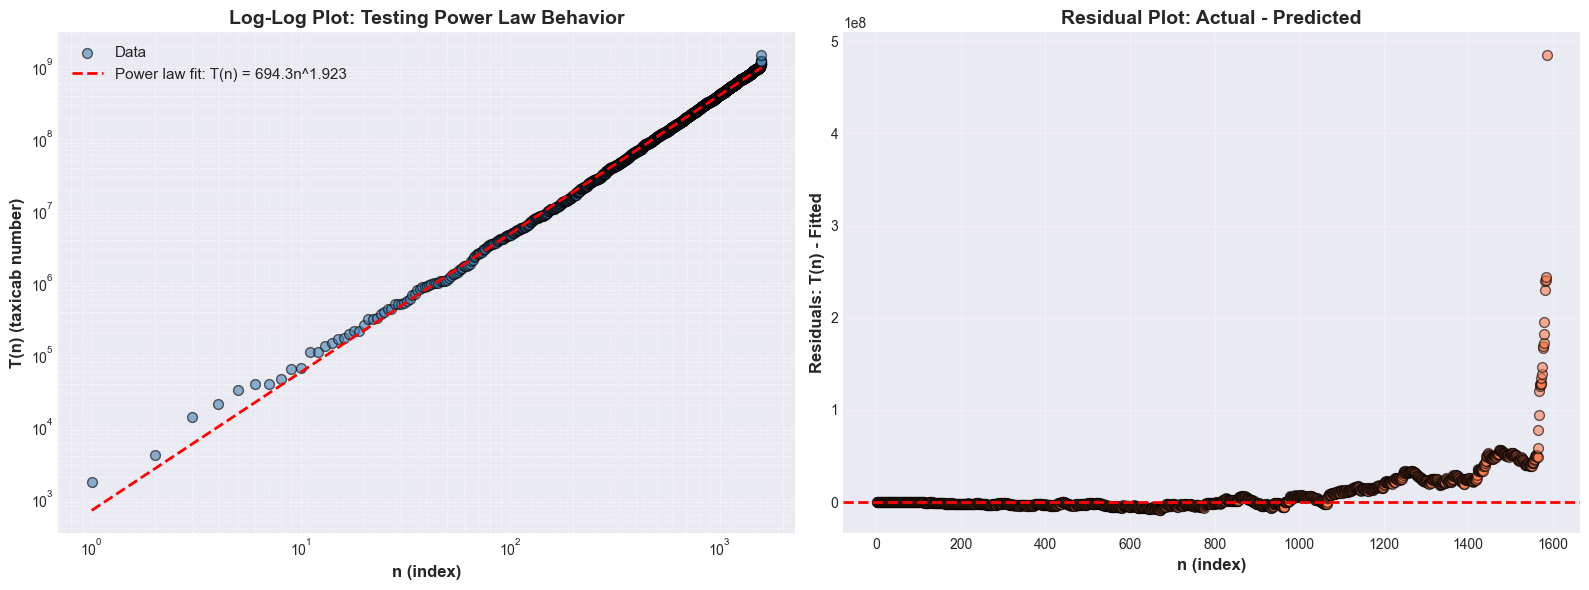
\includegraphics[width=0.95\textwidth]{powerlaw_plot.png}
  \caption{Log--log plot of taxicab numbers with fitted power-law model $T(n) \approx 694.34\,n^{1.923}$ (left), and residuals $T(n) - cn^{\alpha}$ as a function of index (right).}
  \label{fig:powerlaw}
\end{figure}

To test the tightness of our $O(X^{2/3})$ bound, we computed $S(X)$ empirically for large values of $X$ and plotted $\log S(X)$ against $\log X$. On a log-log scale, $S(X) \propto X^k$ appears as a line of slope $k$. Our theoretical bound predicts slope at most $2/3 \approx 0.667$, but a linear fit to the empirical data yields a slope of approximately $0.510$, as shown in Figure~\ref{fig:density}.

\begin{figure}[ht]
  \centering
  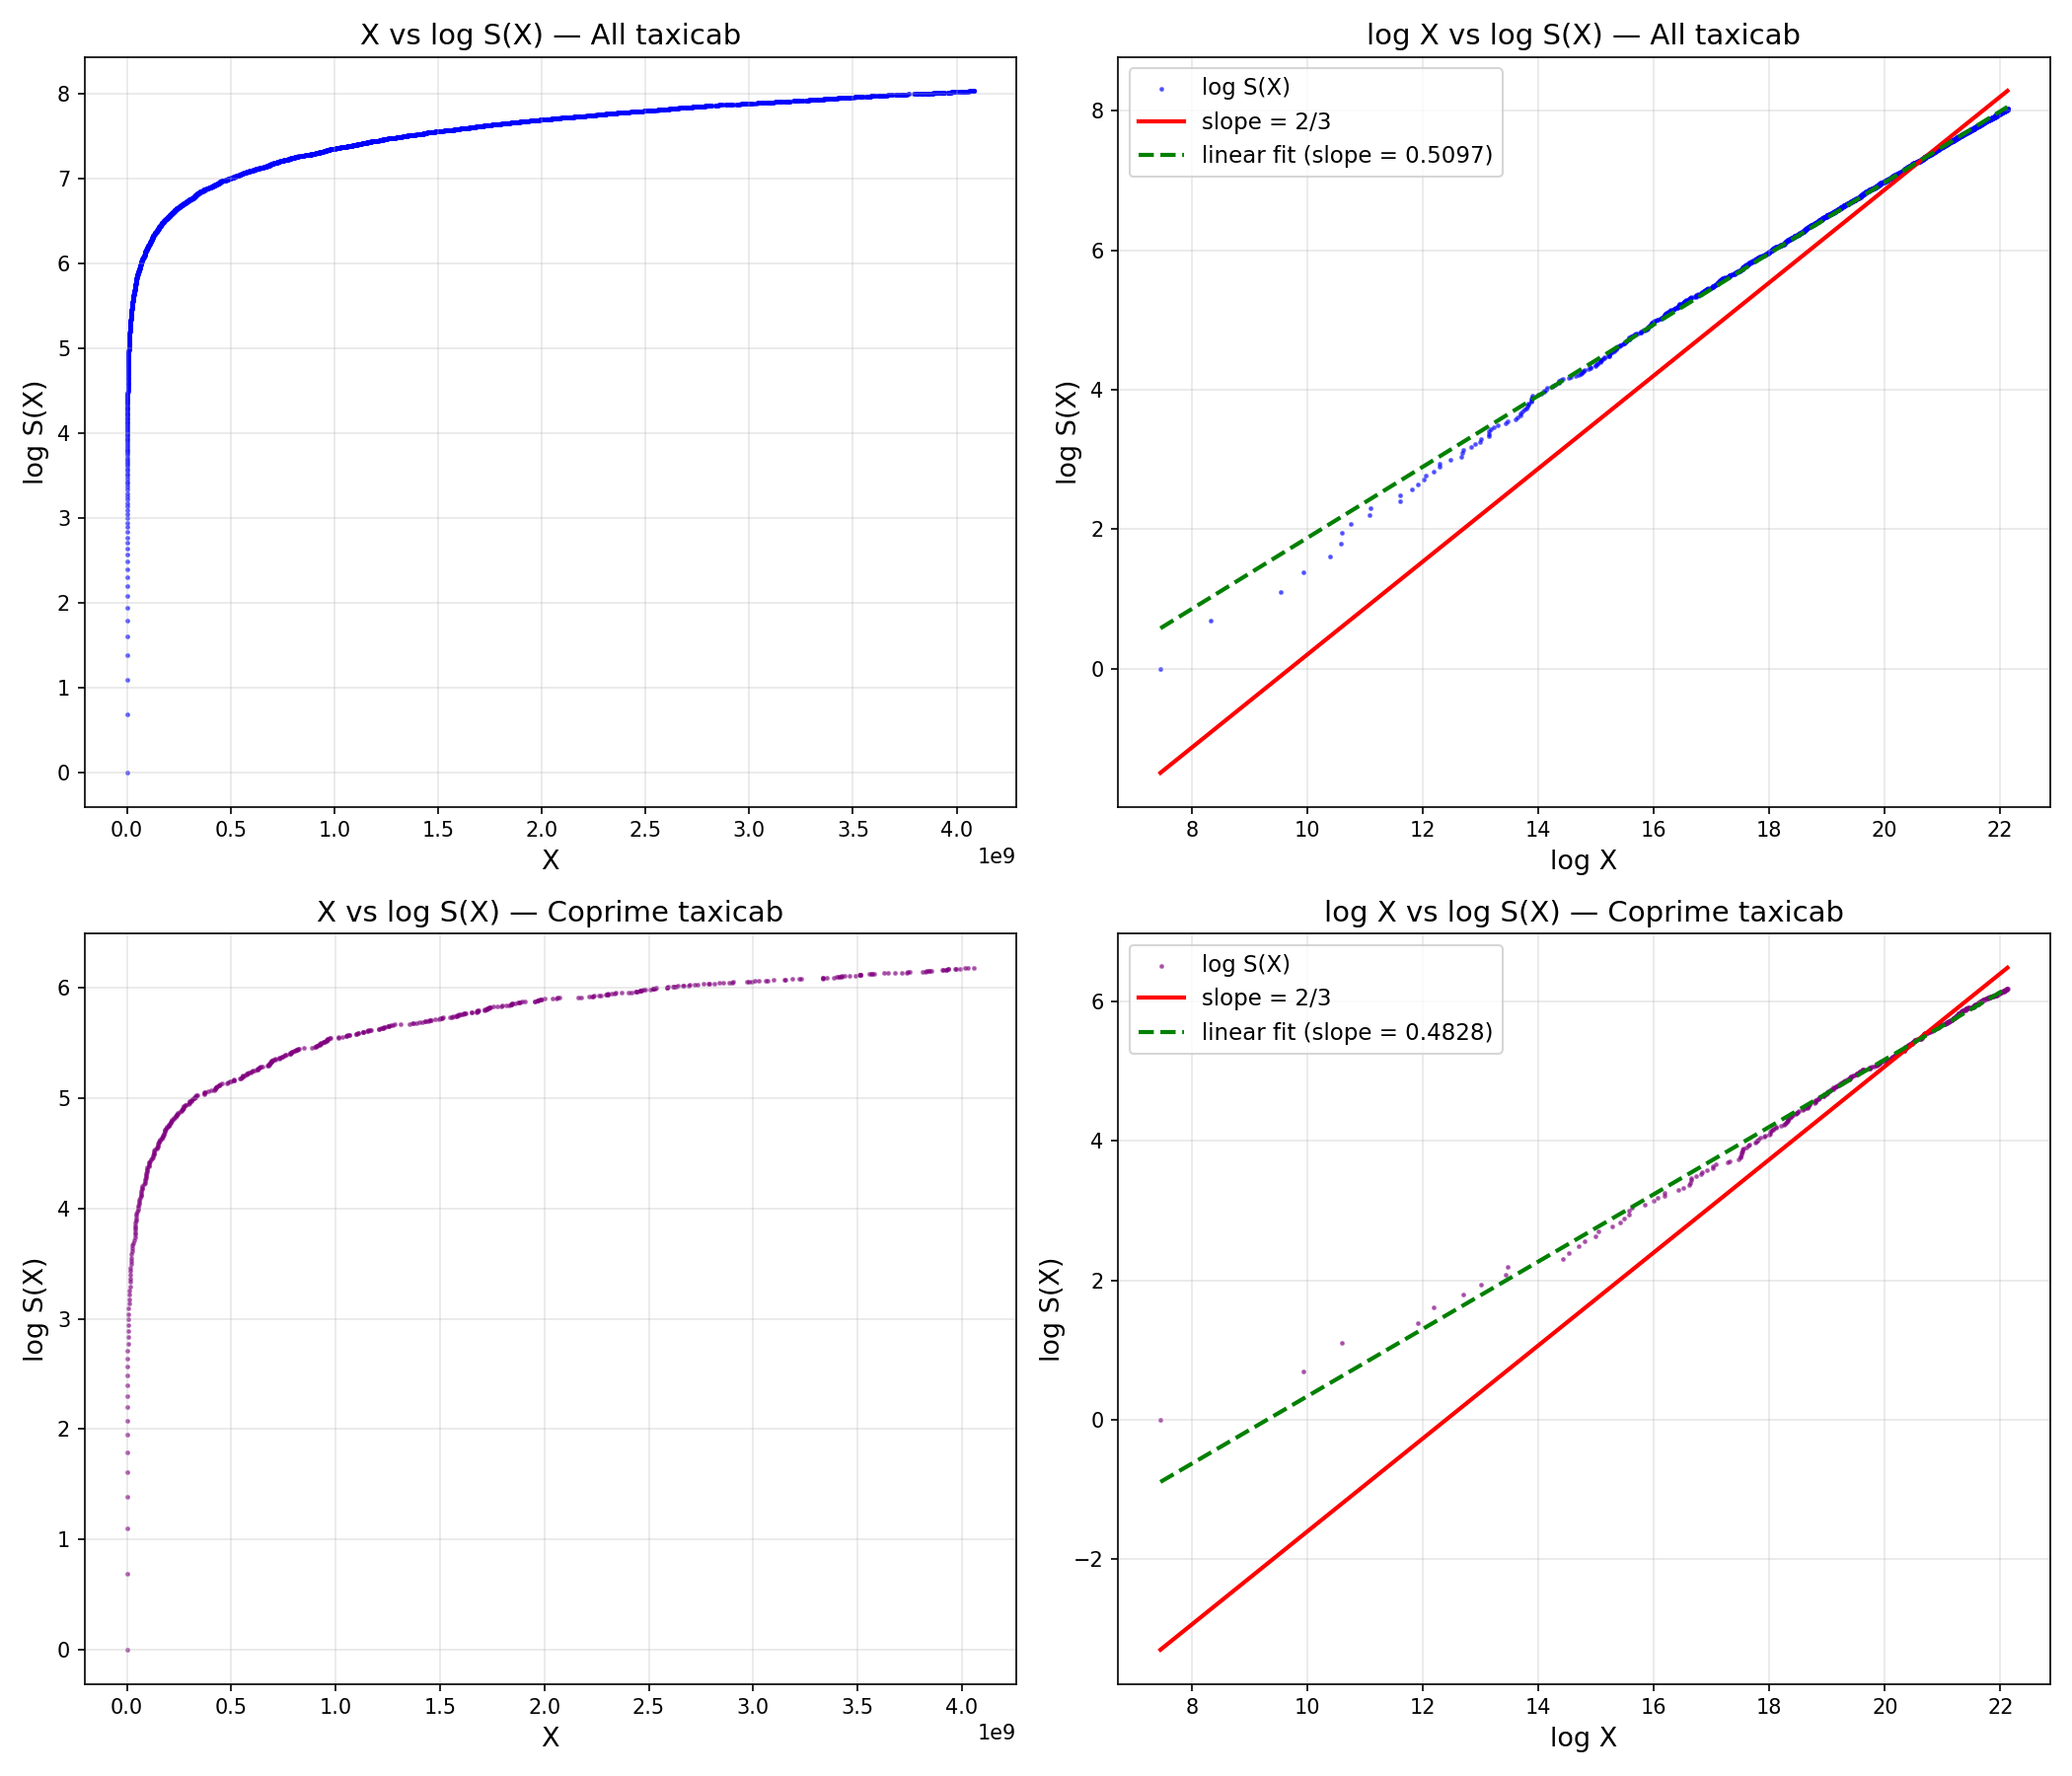
\includegraphics[width=0.95\textwidth]{taxicab_density_plot.png}
  \caption{Empirical growth of $S(X)$ (top row) and $S_{\mathrm{nt}}(X)$ (bottom row). The left column plots $X$ vs the respective counting function; the right column plots both on a log--log scale. In each log--log plot, the solid red line is the theoretical $O(X^{2/3})$ bound (slope $2/3$) and the dashed green line is the empirical best fit. The fitted slopes are approximately $0.510$ for all taxicab numbers and $0.483$ for non-trivially related taxicab numbers.}
  \label{fig:density}
\end{figure}

This suggests that the true growth rate of $S(X)$ is significantly slower than our proven upper bound of $O(X^{2/3})$. In particular, the empirical slope of $0.510$ is much closer to $1/2$ than to $2/3$, and remains stable across the range of data we tested. This leads us to the following conjecture.

\begin{conjecture}\label{conj:density}
  $S(X) = \Theta(X^{1/2})$.
\end{conjecture}

Combined with the lower bound $S(X) = \Omega(X^{1/3})$ from Theorem~\ref{thm:growth}, this would place the true growth rate of taxicab numbers between $X^{1/3}$ and $X^{2/3}$, with our empirical data suggesting it is near the upper end.
\newline

A probabilistic heuristic can offer additional insight here. There are $R(X) \approx X^{2/3}$ representations of integers up to $X$ as sums of two cubes, distributed among roughly $X$ possible values. If these representations were distributed uniformly at random, a birthday-paradox calculation predicts approximately $\binom{R(X)}{2} \cdot \frac{1}{X} \approx \frac{X^{1/3}}{2}$ collisions---integers with at least two representations. This gives a heuristic lower bound of $\Omega(X^{1/3})$, consistent with our proven bound. The discrepancy between this heuristic ($X^{1/3}$) and the empirical exponent ($\approx X^{1/2}$) suggests that sums of two cubes are not uniformly distributed: certain values are more likely to admit multiple representations, a phenomenon plausibly explained by the modular structure we analyze in Section~\ref{sec:modular}.
\newline

The preceding bounds count all taxicab numbers, including those that arise as rescalings of smaller ones via Lemma~\ref{lem:scaling}. We now restrict attention to non-trivially related taxicab numbers and let $S_{\mathrm{nt}}(X)$ denote their count up to $X$.

\begin{theorem}\label{thm:nt-upper}
  $S_{\mathrm{nt}}(X) = O(X^{2/3})$. More precisely, $S_{\mathrm{nt}}(X) \le \frac{3}{2\pi^2}\, X^{2/3}$ for sufficiently large $X$.
\end{theorem}

\begin{proof}
Let $R_{\mathrm{nt}}(X)$ denote the number of coprime pairs $(a,b) \in \mathbb{N}^2$ with $1 \le a \le b$, $\gcd(a,b) = 1$, and $a^3 + b^3 \le X$. As in the proof of Theorem~\ref{thm:density}, every valid pair satisfies $b \le \lfloor X^{1/3} \rfloor$. For a given $b$, the number of integers $a$ with $1 \le a \le b$ and $\gcd(a,b) = 1$ is at most $\phi(b)$, Euler's totient function. Therefore
\[
  R_{\mathrm{nt}}(X) \le \sum_{b=1}^{\lfloor X^{1/3} \rfloor} \phi(b).
\]
The well-known asymptotic $\sum_{b=1}^{k} \phi(b) \sim \frac{3}{\pi^2}\, k^2$ gives
\[
  R_{\mathrm{nt}}(X) \le \frac{3}{\pi^2}\, X^{2/3} + o(X^{2/3}).
\]
Since every non-trivially related taxicab number requires at least two coprime pairs, $2\,S_{\mathrm{nt}}(X) \le R_{\mathrm{nt}}(X)$, and hence $S_{\mathrm{nt}}(X) \le \frac{3}{2\pi^2}\, X^{2/3}$ for sufficiently large $X$.
\end{proof}

The constant $\frac{3}{2\pi^2} \approx 0.152$ is smaller than the constant $\frac{1}{2}$ in Theorem~\ref{thm:density}, reflecting the sparsity of coprime pairs among all pairs. For the lower bound, the scaling argument of Theorem~\ref{thm:growth} is unavailable: the family $\{1729\,t^3\}$ produces representations with $\gcd(ta,tb) = t$, which are trivially related for $t \ge 2$. Instead, we appeal to the parametric family of Section~\ref{sec:infinite}.

\begin{theorem}\label{thm:nt-lower}
  $S_{\mathrm{nt}}(X) = \Omega(X^{1/9})$.
\end{theorem}

\begin{proof}
By Lemma~\ref{thm:family}, each positive integer $n$ produces a taxicab number $N(n) = r_n^3 + s_n^3$ with largest base $r_n = 9n^3 + 6n^2 + 1$. Since $r_n \sim 9n^3$, we have $N(n) \sim 729\,n^9$, so the condition $N(n) \le X$ is satisfied whenever $n \le (X/729)^{1/9}$. By Lemma~\ref{lem:nontrivial}, no two members of this family are trivially related. Hence
\[
  S_{\mathrm{nt}}(X) \ge \left\lfloor \left(\frac{X}{729}\right)^{1/9} \right\rfloor = \Omega(X^{1/9}).
\]
\end{proof}

The proven bounds $\Omega(X^{1/9}) \le S_{\mathrm{nt}}(X) \le O(X^{2/3})$ leave a wider gap than for all taxicab numbers. Empirically, a log--log fit for $S_{\mathrm{nt}}(X)$ yields a slope of approximately $0.483$ (see the bottom row of Figure~\ref{fig:density}), close to $1/2$ and well within the proven range.

\section{Modular Structure of Sums of Powers}\label{sec:modular}
A natural approach to understanding which integers can be Taxicab numbers
is to ask, for each modulus $m$, which residue classes modulo $m$ contain
at least one sum of two cubes. Any integer whose residue modulo $m$ falls
outside the achievable classes is immediately disqualified as a Taxicab
number, regardless of its other properties. We develop this idea in two
stages. In \S\ref{subsec:mod63} we derive constraints on the residues of
$a^3 + b^3$ modulo $9$, and $7$, and combine the constraints
via the Chinese Remainder Theorem to produce a sieve
modulo $63$ that eliminates $38$ out of $63$ residue classes modulo $63$ from
containing any sum of two cubes. In \S\ref{subsec:optimal} we ask whether this excluded fraction of
$38/63$ is the best achievable over all moduli. Using the achievable
fraction $f(m)$ introduced in Definition~\ref{def:achievable} and the
prime power raising result of Proposition~\ref{prop:lifting} and
Theorem~\ref{thm:lifting-general}, we prove in Theorem~\ref{thm:mod63}
that that no modulus whose prime 
factors are drawn from $\{3, 7\}$ together with any
prime $p \equiv 2 \pmod{3}$ can improve upon the excluded fraction $38/63$. We conclude with Conjecture~\ref{conj:optimal}, supported by
computational verification up to $p = 10{,}000$, that $38/63$ is in
fact optimal over all moduli.

\subsection{The modulo-63 sieve for sums of two cubes}\label{subsec:mod63}

The strategy employed in this section is to identify residue classes modulo small
prime powers that no sum of two cubes can occupy. Each such exclusion
immediately disqualifies infinitely many integers from being Taxicab
numbers. 

We begin at the prime power $9$, where a direct expansion determines the
cube residues completely.

\begin{lemma}\label{lem:cubes-mod9}
For every integer $n$, $n^3 \bmod 9 \in \{0, 1, 8\}$. Consequently, the
achievable residues of $a^3 + b^3 \pmod{9}$ are exactly $\{0,1,2,7,8\}$,
and the four residue classes $\{3,4,5,6\}$ are excluded.
\end{lemma}

\begin{proof}
Every integer $n$ satisfies $n \equiv 0$, $1$, or $2 \pmod{3}$, so we
write $n = 3q + r$ with $r \in \{0, 1, 2\}$ and expand:
\begin{align*}
r = 0: &\quad n^3 = 27q^3 \equiv 0 \pmod{9},\\
r = 1: &\quad n^3 = 27q^3 + 27q^2 + 9q + 1 \equiv 1 \pmod{9},\\
r = 2: &\quad n^3 = 27q^3 + 54q^2 + 36q + 8 \equiv 8 \pmod{9}.
\end{align*}
The cube residues modulo $9$ are therefore $\{0, 1, 8\} = \{0, +1, -1\}$.
Since $a^3$ and $b^3$ each lie in this set, the nine possible pairwise
sums are $\{0+0, 0+1, 0+8, 1+0, 1+1, 1+8, 8+0, 8+1, 8+8\}$, which
reduce modulo $9$ to $\{0, 1, 2, 7, 8\}$.
\end{proof}

The same approach applies modulo $7$: we determine all possible 
values of $n^3 \bmod 7$ by applying Fermat's Little Theorem, 
enumerate the pairwise sums of those values, and identify the 
residue classes that no sum of two cubes can occupy.

\begin{lemma}\label{lem:cubes-mod7}
For every integer $n$, $n^3 \bmod 7 \in \{0, 1, 6\}$. Consequently, the
achievable residues of $a^3 + b^3 \pmod{7}$ are exactly $\{0,1,2,5,6\}$,
and the two residue classes $\{3,4\}$ are excluded.
\end{lemma}

\begin{proof}
By Fermat's Little Theorem, $n^6 \equiv 1 \pmod{7}$ for $7 \nmid n$.
Since $n^6 = (n^3)^2$, this means $n^3$ is a square root of $1$ modulo
$7$. As $x^2 - 1 = (x-1)(x+1)$ has no zero divisors modulo the prime
$7$, the only square roots of $1$ are $\pm 1$, giving $n^3 \equiv 1$ or
$6 \pmod{7}$. Including $n \equiv 0$, the cube residues modulo $7$ are
$\{0, 1, 6\} = \{0, +1, -1\}$. The pairwise sums of elements of this
set are $\{0, 1, 2, 5, 6\}$ modulo $7$, so $\{3, 4\}$ are excluded.
\end{proof}

Before combining these constraints via the Chinese Remainder Theorem, 
it is useful to introduce a quantity that measures how much of the 
integer line each modulus rules out as sums of two cubes.

\begin{definition}\label{def:achievable}
For a positive integer $m$, let
\[
  A_m = \{r \bmod m : a^3 + b^3 \equiv r \pmod{m}
  \text{ for some integers } a, b\}
\]
be the set of achievable residues modulo $m$. This is precisely the set
of residue classes that are not ruled out as sums of two cubes by
arithmetic modulo $m$ alone: any integer whose residue modulo $m$ does
not lie in $A_m$ cannot be a sum of two cubes, and hence cannot be a
Taxicab number. The achievable fraction $f(m) = |A_m|/m$ measures what
proportion of residue classes survive this test. A smaller value of
$f(m)$ corresponds to a stronger sieve: $f(m) = 1$ means modulus $m$
provides no restriction whatsoever, while $f(m) = 25/63$ means that over
$60\%$ of all integers are immediately excluded from consideration.
\end{definition}

Using this definition, Lemma~\ref{lem:cubes-mod9} gives $f(9) = 5/9$, since
exactly $5$ of the $9$ residue classes modulo $9$ are achievable as sums
of two cubes. To see this directly: the cube residues modulo $9$ are
$\{0, 1, 8\}$, and the $3 \times 3$ table of pairwise sums produces
exactly $5$ distinct values $\{0, 1, 2, 7, 8\}$ modulo $9$, confirming
$|A_9| = 5$ and hence $f(9) = 5/9$. Similarly,
Lemma~\ref{lem:cubes-mod7} gives $f(7) = 5/7$: the cube residues modulo
$7$ are $\{0, 1, 6\}$, whose $3 \times 3$ table of pairwise sums produces
exactly $5$ distinct values $\{0, 1, 2, 5, 6\}$ modulo $7$, giving
$|A_7| = 5$ and $f(7) = 5/7$.
\medskip

Having established the achievable fractions $f(9) = 5/9$ and 
$f(7) = 5/7$ from Lemmas~\ref{lem:cubes-mod9} 
and~\ref{lem:cubes-mod7}, we now combine them via the Chinese 
Remainder Theorem to produce the modulo-$63$ sieve.

\begin{theorem}\label{thm:sieve63}
At least $38$ of the $63$ residue classes modulo $63$ contain no sum 
of two cubes, and therefore no Taxicab number. 
\end{theorem}

\begin{proof}
Since $63 = 9 \times 7$ and $\gcd(9,7) = 1$, the Chinese Remainder 
Theorem establishes that specifying a residue class modulo $63$ is 
equivalent to independently specifying a residue class modulo $9$ and 
a residue class modulo $7$: every pair $(r_1 \bmod 9,\, r_2 \bmod 7)$ 
corresponds to exactly one residue class modulo $63$, and every 
residue class modulo $63$ arises from exactly one such pair. By 
Lemma~\ref{lem:cubes-mod9}, any sum $N = a^3 + b^3$ must satisfy 
$N \bmod 9 \in \{0,1,2,7,8\}$, and by Lemma~\ref{lem:cubes-mod7} it 
must satisfy $N \bmod 7 \in \{0,1,2,5,6\}$. Since these two 
constraints operate at coprime moduli they are independent, so the 
residue classes modulo $63$ that can contain a sum of two cubes 
correspond exactly to pairs in the Cartesian product 
$\{0,1,2,7,8\} \times \{0,1,2,5,6\}$, which has $5 \times 5 = 25$ 
elements. Therefore at most $25$ residue classes modulo $63$ are 
achievable, giving $f(63) \le 25/63$ and at least $63 - 25 = 38$ 
excluded classes. 
\end{proof}

Lemma \ref{lem:f-multiplicative} below makes this argument precise for general coprime moduli.

\subsection{Optimality of the modulo-63 sieve}\label{subsec:optimal}
Theorem~\ref{thm:sieve63} establishes that the modulo-$63$ sieve 
excludes a fraction $38/63$ of all residue classes. A natural question 
is whether this fraction can be improved by a larger 
modulus.

\medskip
A residue class modulo $3^k$ is a set of integers all 
having the same remainder when divided by $3^k$. There are $3^k$ such 
classes, and each one is entirely contained within exactly one of the 
nine residue classes modulo $9$, since any two integers with the same 
remainder modulo $3^k$ also have the same remainder modulo $9$. The 
question is therefore whether every residue class modulo $3^k$ that 
is contained in an achievable class modulo $9$, one whose remainder 
modulo $9$ lies in $\{0,1,2,7,8\}$, is itself achievable as a sum 
of two cubes modulo $3^k$, or whether some of these finer classes 
fail to contain any sum of two cubes even though their containing 
class modulo $9$ does. We prove that no such failure occurs: every 
residue class modulo $3^k$ whose remainder modulo $9$ lies in 
$\{0,1,2,7,8\}$ is itself achievable as a sum of two cubes modulo 
$3^k$. The analogous statement holds for powers of $7$: every 
residue class modulo $7^k$ whose remainder modulo $7$ lies in 
$\{0,1,2,5,6\}$ is achievable as a sum of two cubes modulo $7^k$, 
so that the five excluded classes modulo $7$ remain the only excluded 
classes at every higher power of $7$ as well.

\medskip
The following proposition provides the key mechanism for establishing that 
achievability is preserved at higher prime powers. Specifically, it shows that any solution modulo $p^k$ 
can be used to produce a solution in any desired residue class modulo 
$p^{k+1}$, so that no residue class achievable modulo $p^k$ fails 
to be achievable modulo $p^{k+1}$.

\begin{proposition}[Generating solutions to higher prime powers]
\label{prop:lifting}
Let $p$ be an odd prime with $p \ne 3$, let $k \ge 1$, and suppose
$a^3 + b^3 \equiv n \pmod{p^k}$ with $p \nmid a$. Then for every
$t \in \{0, 1, \ldots, p-1\}$ there exists $u \in \{0, 1, \ldots, p-1\}$
such that
\[
(a + up^k)^3 + b^3 \equiv n + tp^k \pmod{p^{k+1}}.
\]
\end{proposition}

\begin{proof}
We expand $(a + up^k)^3$ by the binomial theorem:
\[
(a + up^k)^3 = a^3 + 3a^2(up^k) + 3a(up^k)^2 + (up^k)^3.
\]
The last two terms carry factors of $p^{2k}$ and $p^{3k}$ respectively.
Since $k \ge 1$, both $2k \ge k+1$ and $3k \ge k+1$, so both terms
vanish modulo $p^{k+1}$. Therefore
\[
(a + up^k)^3 + b^3 \equiv a^3 + 3a^2 u\, p^k + b^3
= (a^3 + b^3) + 3a^2 u\, p^k \pmod{p^{k+1}}.
\]
Write $a^3 + b^3 = n + sp^k$ for some integer $s$. Substituting, the
congruence $(a + up^k)^3 + b^3 \equiv n + tp^k \pmod{p^{k+1}}$ becomes
\[
n + sp^k + 3a^2 u\, p^k \equiv n + tp^k \pmod{p^{k+1}},
\]
which simplifies to the linear congruence $s + 3a^2 u \equiv t \pmod{p}$.
Since $p \ne 3$ we have $p \nmid 3$, and since $p \nmid a$ by hypothesis
we have $p \nmid a^2$; therefore the coefficient $3a^2$ is invertible
modulo $p$, and the congruence has a unique solution $u \pmod{p}$, which
we may take in $\{0, 1, \ldots, p-1\}$.
\end{proof}

An example usage of this proposition would be finding a solution to
$a^3 + b^3 \equiv 7 \pmod{25}$. Since $7 \equiv 2 \pmod{5}$, we first
find a base solution modulo $5$: take $b = 1$ and solve
$a^3 \equiv 1 \pmod{5}$, giving $a = 1$, so $1^3 + 1^3 = 2 \equiv 2
\pmod{5}$. Writing $7 = 2 + 5 \cdot 1$, we have $s = 0$ and $t = 1$.
Proposition~\ref{prop:lifting} requires solving
$0 + 3 \cdot 1^2 \cdot u \equiv 1 \pmod{5}$, that is $3u \equiv 1
\pmod{5}$, giving $u \equiv 2 \pmod{5}$. Setting $a' = 1 + 5 \cdot 2 =
11$, we verify:
\[
11^3 + 1^3 = 1331 + 1 = 1332 = 53 \cdot 25 + 7 \equiv 7 \pmod{25}.
\]

The proposition requires $p \nmid a$ in the existing solution in order 
to guarantee that the coefficient $3a^2$ is invertible modulo $p$, 
making the adjustment uniquely solvable. The following theorem shows 
that whenever $f(p) = 1$, every residue class modulo $p$ admits a 
representation with $p \nmid a$, so that the proposition can be applied 
at every stage of an induction on $k$. 

\begin{theorem}\label{thm:lifting-general}
Let $p$ be an odd prime with $p \ne 3$, and let $k \ge 1$ be a positive 
integer. If $f(p) = 1$, then $f(p^k) = 1$.
\end{theorem}
\begin{proof}
We prove by induction on $k$ that every residue class $T \pmod{p^k}$ 
has a representation $a^3 + b^3 \equiv T \pmod{p^k}$ with $p \nmid a$. When $k = 1$, the assumption $f(p) = 1$ guarantees every 
residue class modulo $p$ is achievable, and we verify that each admits 
a representation with $p \nmid a$: for $T \not\equiv 0 \pmod{p}$, if a 
given solution has $p \mid a$, then $a^3 + b^3 \equiv T \not\equiv 0$ 
forces $p \nmid b$, and relabeling $a \leftrightarrow b$ gives the 
required representation; for $T \equiv 0 \pmod{p}$, the representation 
$a = 1$, $b = -1$ gives $1^3 + (-1)^3 = 0$ with $p \nmid 1$.

Now suppose the claim holds for some $k \ge 1$, so that every residue 
class modulo $p^k$ has a representation with $p \nmid a$. Let $T$ be 
any residue class modulo $p^{k+1}$, and write 
$T \equiv t + \delta p^k \pmod{p^{k+1}}$ where $t = T \bmod p^k$ and 
$\delta \in \{0, \ldots, p-1\}$. The inductive hypothesis supplies 
integers $a, b$ with $p \nmid a$ and $a^3 + b^3 \equiv t \pmod{p^k}$, 
and since $p \nmid a$, Proposition~\ref{prop:lifting} yields 
$u \in \{0, \ldots, p-1\}$ such that 
$(a + up^k)^3 + b^3 \equiv T \pmod{p^{k+1}}$. Since 
$a + up^k \equiv a \not\equiv 0 \pmod{p}$, the condition $p \nmid a$ 
is preserved, completing the induction.
\end{proof}

Theorem~\ref{thm:lifting-general} applies whenever $f(p) = 1$ can be
verified at the prime itself. We now establish the achievable fractions
for each prime relevant to our sieve, beginning with the two cases to
which the theorem applies directly.

\begin{lemma}\label{lem:f-p2mod3}
If $p \equiv 2 \pmod{3}$ and $p \ne 3$, and $k \ge 1$ is a positive 
integer, then $f(p^k) = 1$.
\end{lemma}

\begin{proof}
The multiplicative group $(\mathbb{Z}/p\mathbb{Z})^*$ consists of the
nonzero residues modulo $p$ under multiplication. Since $p$ is prime,
this group is cyclic of order $p - 1$. In a cyclic group of order $n$,
the map $x \mapsto x^j$ is a bijection if and only if $\gcd(j, n) = 1$.
Here $j = 3$ and $n = p - 1$; since $p \equiv 2 \pmod{3}$, we have
$p - 1 \equiv 1 \pmod{3}$, so $\gcd(3, p-1) = 1$. Therefore the cubing
map is a bijection on $(\mathbb{Z}/p\mathbb{Z})^*$, meaning every nonzero
residue modulo $p$ is a perfect cube. Together with $0^3 = 0$, every
residue class modulo $p$ is achievable as a cube.

It follows that for any target $t \in \mathbb{Z}/p\mathbb{Z}$, we may
take $b = 1$ and observe that $a^3 \equiv t - 1 \pmod{p}$ is solvable,
since $t - 1$ is a residue modulo $p$ and every residue is a cube. This
gives $a^3 + b^3 \equiv t \pmod{p}$ with $p \nmid b = 1$, so $f(p) = 1$.
Theorem~\ref{thm:lifting-general} then yields $f(p^k) = 1$ for all
$k \ge 1$.
\end{proof}

\begin{lemma}\label{lem:f-7}
For every positive integer $k \ge 1$, $f(7^k) = 5/7$.
\end{lemma}

\begin{proof}
By Lemma~\ref{lem:cubes-mod7}, the achievable residues modulo $7$ are 
exactly $\{0,1,2,5,6\}$, giving $f(7) = 5/7$. To apply 
Proposition~\ref{prop:lifting} and extend each base case to all higher 
powers of $7$, we require a representation with $7 \nmid a$ for each 
of the five achievable classes:
\begin{align*}
r = 0: &\quad a = 1,\ b = 6,\quad 1 + 216 = 217 \equiv 0 \pmod{7},\\
r = 1: &\quad a = 1,\ b = 0,\quad 1 + 0 = 1,\\
r = 2: &\quad a = 1,\ b = 1,\quad 1 + 1 = 2,\\
r = 5: &\quad a = 3,\ b = 3,\quad 27 + 27 = 54 \equiv 5 \pmod{7},\\
r = 6: &\quad a = 3,\ b = 0,\quad 27 + 0 = 27 \equiv 6 \pmod{7}.
\end{align*}
In each case $7 \nmid a$. Since $7 \ne 3$, 
Proposition~\ref{prop:lifting} applies to each of these five base 
cases, extending every achievable class modulo $7$ to all higher powers 
$7^k$. Therefore $f(7^k) = 5/7$ for all $k \ge 1$.
\end{proof}

The case $p = 3$ requires a different approach, since
Proposition~\ref{prop:lifting} explicitly excludes it. The obstruction
is that $3 \mid 3a^2$ regardless of $a$, so the coefficient $3a^2$ is
never invertible modulo $3$, and the argument used for $p = 7$ is
unavailable. A different perturbation must be employed.

\begin{lemma}\label{lem:f-3}
$f(3) = 1$ and, for every integer $k \ge 2$, $f(3^k) = 5/9$.
\end{lemma}

\begin{proof}
Every integer satisfies $n \equiv 0$, $1$, or $2 \pmod{3}$, and a direct
check gives $0^3 \equiv 0$, $1^3 \equiv 1$, $2^3 \equiv 8 \equiv 2
\pmod{3}$, so $n^3 \equiv n \pmod{3}$ for all $n$. Therefore
$a^3 + b^3 \equiv a + b \pmod{3}$, and since $a + b$ ranges over all
residues modulo $3$, every residue class is achievable as a sum of two
cubes, giving $f(3) = 1$.  For
$k \ge 2$, the upper bound $f(3^k) \le 5/9$ follows from
Lemma~\ref{lem:cubes-mod9}: any class excluded modulo $9$ remains
excluded modulo $3^k$, since $9 \mid 3^k$ and reduction modulo $9$ is
well-defined.

For the lower bound, we prove by induction on $k \ge 2$ that every
residue class $T \pmod{3^k}$ with $T \bmod 9 \in \{0,1,2,7,8\}$ has a
representation $a^3 + b^3 \equiv T \pmod{3^k}$ with $3 \nmid b$. The
base case $k = 2$ is established by explicit construction:
\begin{align*}
r = 0: &\quad a = 1,\ b = 2,\quad 1 + 8 = 9 \equiv 0 \pmod{9},\\
r = 1: &\quad a = 0,\ b = 1,\quad 0 + 1 = 1,\\
r = 2: &\quad a = 1,\ b = 1,\quad 1 + 1 = 2,\\
r = 7: &\quad a = 2,\ b = 2,\quad 8 + 8 = 16 \equiv 7 \pmod{9},\\
r = 8: &\quad a = 0,\ b = 2,\quad 0 + 8 = 8.
\end{align*}
In each case $3 \nmid b$. For the inductive step, suppose the claim holds
for some $k \ge 2$: every class $t \pmod{3^k}$ with $t \bmod 9 \in
\{0,1,2,7,8\}$ has a representation $a^3 + b^3 \equiv t \pmod{3^k}$
with $3 \nmid b$. Let $T$ be any residue class modulo $3^{k+1}$ with
$T \bmod 9 \in \{0,1,2,7,8\}$, and write $T \equiv t + \delta \cdot 3^k
\pmod{3^{k+1}}$ where $t = T \bmod 3^k$ and $\delta \in \{0,1,2\}$.
Since $t \bmod 9 = T \bmod 9 \in \{0,1,2,7,8\}$, the inductive
hypothesis supplies integers $a, b$ with $3 \nmid b$ and
$a^3 + b^3 \equiv t \pmod{3^k}$.

Set $b' = b + u \cdot 3^{k-1}$ for some $u \in \{0,1,2\}$ to be
determined. Expanding by the binomial theorem,
\[
(b')^3 = b^3 + 3b^2(u \cdot 3^{k-1}) + 3b(u \cdot 3^{k-1})^2
+ (u \cdot 3^{k-1})^3.
\]
For $k \ge 2$, the last two terms are divisible by $3^{2k-1}$ and
$3^{3(k-1)}$ respectively; since both $2k-1 \ge k+1$ and
$3(k-1) \ge k+1$ hold for $k \ge 2$, these terms vanish modulo
$3^{k+1}$. Therefore
\[
a^3 + (b')^3 \equiv t + u b^2 \cdot 3^k \pmod{3^{k+1}}.
\]
For this expression to equal $T \equiv t + \delta \cdot 3^k
\pmod{3^{k+1}}$, we require $u b^2 \equiv \delta \pmod{3}$. Since
$3 \nmid b$, we have $b^2 \equiv 1 \pmod{3}$, so this reduces to
$u \equiv \delta \pmod{3}$, which has the explicit solution $u = \delta$.
Finally, $b' \equiv b \pmod{3}$ and $3 \nmid b$ together give
$3 \nmid b'$, preserving the inductive condition. Therefore, by induction,
$f(3^k) = 5/9$ for all $k \ge 2$.
\end{proof}

With the achievable fractions at all relevant prime powers established,
we now combine them into a single optimal sieve, which motivates the following lemma. 

\begin{lemma}\label{lem:f-multiplicative}
If $\gcd(m_1, m_2) = 1$, then $f(m_1 m_2) = f(m_1) \cdot f(m_2)$.
\end{lemma}

\begin{proof}
Since $\gcd(m_1, m_2) = 1$, the Chinese Remainder Theorem gives a 
bijection between residue classes modulo $m_1 m_2$ and pairs of 
residue classes $(r_1 \bmod m_1,\, r_2 \bmod m_2)$. A class 
$r \bmod m_1 m_2$ is achievable as a sum of two cubes if and only if 
both $r \bmod m_1 \in A_{m_1}$ and $r \bmod m_2 \in A_{m_2}$, since 
a solution modulo $m_1 m_2$ reduces to solutions modulo $m_1$ and 
$m_2$ separately, and conversely any pair of solutions modulo $m_1$ 
and $m_2$ lifts uniquely to a solution modulo $m_1 m_2$ by the Chinese 
Remainder Theorem. Therefore $|A_{m_1 m_2}| = |A_{m_1}| \cdot 
|A_{m_2}|$, and dividing by $m_1 m_2 = m_1 \cdot m_2$ gives 
$f(m_1 m_2) = f(m_1) \cdot f(m_2)$.
\end{proof}

Applying this lemma to the constraints found moduli $9$, $7$, and $p \equiv 2 \mod(3) $ yields the main result of this section.

\begin{theorem}\label{thm:mod63}
The achievable fraction $f(63) = 25/63$ established in 
Theorem~\ref{thm:sieve63} cannot be reduced by passing to any modulus 
of the form $3^j \cdot 7^k$. Any further reduction of the achievable 
fraction requires introducing a prime $p \equiv 1 \pmod{3}$ with 
$p > 7$ into the modulus.
\end{theorem}

\begin{proof}
By Lemmas~\ref{lem:f-3} and~\ref{lem:f-7}, $f(3^j) = 5/9$ for all 
$j \ge 2$ and $f(7^k) = 5/7$ for all $k \ge 1$. By 
Lemma~\ref{lem:f-multiplicative}, the achievable fraction for any 
modulus of the form $3^j \cdot 7^k$ is therefore 
$(5/9)(5/7) = 25/63$, the same value as at modulus $63$ itself. No 
choice of $j \ge 2$ and $k \ge 1$ reduces this fraction further, so 
the excluded fraction $38/63$ cannot be improved within this family 
of moduli.

For the second claim, consider any modulus whose prime factors include 
primes outside $\{3, 7\}$. By Lemma~\ref{lem:f-p2mod3}, every prime 
$p \equiv 2 \pmod{3}$ satisfies $f(p^k) = 1$, so including such 
primes in the modulus contributes no additional excluded classes. The 
prime $p = 2$ similarly satisfies $f(2^k) = 1$, since every integer 
is a cube modulo $2$. Therefore the only primes that could potentially 
reduce the achievable fraction below $25/63$ are those satisfying 
$p \equiv 1 \pmod{3}$ with $p > 7$. Whether any such prime yields 
$f(p) < 1$ is the subject of Conjecture~\ref{conj:optimal}.
\end{proof}

\begin{conjecture}\label{conj:optimal}
The excluded fraction $38/63$ is optimal over all moduli $m$, not 
merely those built from the primes $3$ and $7$. Equivalently, for 
every prime $p \equiv 1 \pmod{3}$ with $p > 7$, if $C$ denotes the 
set of residues modulo $p$ that are perfect cubes, that is,
\[
C = \{a^3 \bmod p : a \in \{0, 1, \ldots, p-1\}\},
\]
then the sumset $C + C = \{c_1 + c_2 \bmod p : c_1, c_2 \in C\}$ 
equals all of $\{0, 1, \ldots, p-1\}$. This means every residue class 
modulo $p$ is achievable as a sum of two cubes, so that $f(p) = 1$ 
and introducing $p$ into the modulus contributes no additional 
excluded classes to the sieve. This has been verified computationally 
for all primes $p \equiv 1 \pmod{3}$ with $7 < p \le 10{,}000$.
\end{conjecture}
\section{Acknowledgments:}
\begin{itemize}
    \item Jovani: Section 1, 2
    \item Sky: Section 3, 5.1, 5.2
    \item Samir: Section 4
\end{itemize}



\end{document}
